The questionnaire was created mainly to figure out more precise weights for how people choose the media they want to consume. So not only as a way to validate the results from the interviews, but also to determine variables to implement later in a possible solution.
In total, the questionnaire received 82 responses from 52 males and 30 females. The most dominant age group were the 21 to 25 year olds, which represents over half of all the responses. There was an almost even spread between the daily usage of different media, with books being the lowest and movies being the highest.
The questionnaire used a scale from 1 to 5, to rate how high they weigh a certain factor about a media, where 1 is the lowest weight and 5 is the highest weight.

\begin{figure}[htb]
\centering
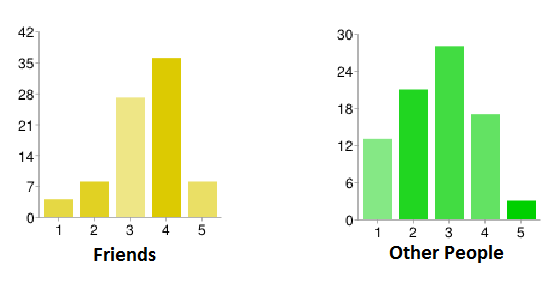
\includegraphics[width=0.8\textwidth]{Images/people.png}
\caption{Graph showing how much people weigh recommendations from their friends and other people}
\label{People}
\end{figure}

\begin{figure}[htb]
\centering
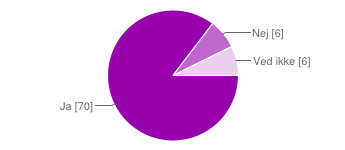
\includegraphics[width=0.8\textwidth]{Images/own.png}
\caption{Graph showing how many people weigh their own opinion highest.}
\label{Own}
\end{figure}

The questionnaire began by asking three questions about how highly they weigh their friends, strangers, and their own opinion when deciding on whether or not to consume a new media. From the responses it was observed that they weigh their friends opinion higher than strangers, with friends getting a 4, and strangers a 3. The total spread can be seen in \ref{People}. In the final of the three questions it was asked if they weigh their own opinion higher than their friends,  the answers showed that they do weigh their own opinion higher than that of their friends when it comes to a new piece of media. Which can be seen in \ref{Own}.

Then the questionnaire went on to ask more specific questions about different media; movies, books, music, and video games. It asked how high they weigh certain features, e.g. the director of a movie. Something that was present through the different types of media, was that the genre had a high weight when picking a new piece of media. Genre was also superior compared to every other feature.
Other more niche features was also evaluated:

\textbf{Movies:}

Features like who directed the movie had a moderately high weight, together with which actors was part of the cast. These two was the most prominent, where the last one was other associated people.

\textbf{Books:}

For books only the author was evaluated. The author had a moderate weight for people, but still seems to be quite important for many people.

\textbf{Music:}

When it comes to music, it seems only the specific performer of the song weights highly, while other associated people have a low weight.

\textbf{Video Games:}

Besides the genre, only which studio made the video game had a high weight. Unlike music and movies, actors and voice actors had a very low weights for video games.

People seems to be looking for trends and details about a piece of media, e.g. the name of a certain actor or actress, a studio, an artist, etc.. Most people seems to favor the more apparent features of media, like the actors in a movie, rather than the more obscure like voice actors in a video game. It is also clear that they weigh their own opinion higher, but still hold other peoples opinions to some regard.